% !TeX program = lualatex
% ============================================================
%  Vorlage Abschlussarbeit
%  Autor: Michael Netter
%
%  Engine : LuaLaTeX
%  Biber  : biber main
% ============================================================
\documentclass[
  12pt,       % Schriftgröße
  a4paper,    % Papierformat
  twoside,    % Zweiseitiger Druck (für Buchbindung)
  openright,  % Kapitel beginnen stets auf einer rechten Seite
  %final       % Alle TODOs unterdrücken (für die Abgabeversion)
]{book}

% ------------------------------------------------------------
%  SPRACHE
% ------------------------------------------------------------
\usepackage[main=ngerman, english]{babel}
% Deutschsprachige Silbentrennung und Bezeichner
% (»Abbildung«, »Tabelle«, »Inhaltsverzeichnis« …)

\usepackage{csquotes}
% Korrekte deutsche Anführungszeichen: \enquote{Text} → „Text"
% Pflichtpaket bei biblatex + ngerman

% ------------------------------------------------------------
%  SCHRIFT  (LuaLaTeX: kein inputenc/fontenc erforderlich)
% ------------------------------------------------------------
\usepackage{fontspec}
% Latin Modern ist der fontspec-Standard – keine weitere Konfiguration nötig.
% Zum Wechseln der Hauptschrift eine der folgenden Zeilen einkommentieren:
% \setmainfont{TeX Gyre Termes}    % Times-ähnlich
% \setmainfont{Libertinus Serif}   % moderner Klassiker

% ------------------------------------------------------------
%  SEITENLAYOUT
% ------------------------------------------------------------
\usepackage[
  a4paper,
  inner         = 3.0cm,   % Innensteg (Bundsteg)
  outer         = 2.5cm,   % Außensteg
  top           = 2.5cm,
  bottom        = 2.5cm,
  bindingoffset = 5mm,     % Zuschlag für Klebebindung
  headheight    = 14pt,    % verhindert fancyhdr-Warnung
]{geometry}

% ------------------------------------------------------------
%  FARBEN
% ------------------------------------------------------------
\usepackage{xcolor}
% Wird u. a. für Zeilennummern in Listings benötigt.
\definecolor{lst_keyword}{RGB}{ 30,  80, 160}   % dunkles Blau
\definecolor{lst_string} {RGB}{ 40, 120,  60}   % dunkles Grün
\definecolor{lst_comment}{RGB}{120, 120, 120}   % mittelgrau
\definecolor{lst_number} {RGB}{150, 150, 150}   % hellgrau (Zeilennummern)
\definecolor{lst_rule}   {RGB}{180, 180, 180}   % Randlinie
\definecolor{lst_bg}     {RGB}{230, 230, 230}   % Hintergrundfarbe

% ------------------------------------------------------------
%  TODO-NOTIZEN  (vor Abgabe alle TODOs entfernen)
% ------------------------------------------------------------
\usepackage[colorinlistoftodos,
  obeyFinal,
  textsize      = scriptsize,
  textwidth     = 2.2cm,
  ]{todonotes}
% Verwendung:  \todo[inline]{Hinweis}
% Mit der Dokumentklassenoption [final] werden alle TODOs
% automatisch unterdrückt – ideal für die Abgabeversion.

% ------------------------------------------------------------
%  MIKROTYPOGRAPHIE
% ------------------------------------------------------------
\usepackage[
  final,           % auch im draft-Modus aktiv
  tracking = true,
  % kerning = true ist nur bei pdfTeX verfügbar, nicht bei LuaLaTeX
]{microtype}
% Verbessert Randausgleich und Grauwert automatisch –
% \sloppy ist damit nicht mehr nötig.

% ------------------------------------------------------------
%  GRAFIK
% ------------------------------------------------------------
\usepackage{graphicx}
% Einbinden von Abbildungen: \includegraphics[width=\textwidth]{dateiname}

\usepackage{subcaption}
% Teilabbildungen nebeneinander (Nachfolger von subfig/subfigure):
%   \begin{subfigure}[b]{0.48\textwidth} ... \end{subfigure}
% Querverweise auf Teilabbildungen:
%   Abbildung~\ref{fig:links}   → »Abbildung 1a«
%   \subref{fig:links}          → »(a)«  (nur Buchstabe, für Bildunterschrift)

% ------------------------------------------------------------
%  TABELLEN
% ------------------------------------------------------------
\usepackage{booktabs}
% Professionelle Tabellenlinien: \toprule, \midrule, \bottomrule
% Kein \hline in wissenschaftlichen Tabellen verwenden!

\usepackage{tabularx}
% Tabellen mit automatisch angepasster Spaltenbreite (X-Spalte)

% ------------------------------------------------------------
%  CODE-LISTINGS
% ------------------------------------------------------------
\usepackage{listings}

% --- Gedeckte, drucktaugliche Farben ----------------------------
% Alle Töne funktionieren sowohl auf Screen als auch im
% Graustufen-Ausdruck: sie unterscheiden sich im Hellwert.
\definecolor{lst_bg}     {RGB}{248, 248, 248}   % sehr helles Grau
\definecolor{lst_keyword}{RGB}{ 30,  80, 160}   % dunkles Blau
\definecolor{lst_string} {RGB}{ 40, 120,  60}   % dunkles Grün
\definecolor{lst_comment}{RGB}{120, 120, 120}   % Mittelgrau
\definecolor{lst_number} {RGB}{160, 160, 160}   % Hellgrau (Zeilennummern)
\definecolor{lst_rule}   {RGB}{200, 200, 200}   % Rahmenfarbe

% --- Basisstil (sprachunabhängig) --------------------------------
\lstdefinestyle{basestyle}{
  backgroundcolor   = \color{lst_bg},
  basicstyle        = \ttfamily\small,
  keywordstyle      = \color{lst_keyword}\bfseries,
  stringstyle       = \color{lst_string},
  commentstyle      = \color{lst_comment}\itshape,
  numbers           = none, % Zeilennummern standardmäßig aus
  numberstyle       = \ttfamily\scriptsize\color{lst_number},
  numbersep         = 8pt,  % Abstand der Zeilennummern zum Code
  frame             = single,
  framerule         = 1pt,
  rulecolor         = \color{lst_rule},
  captionpos        = b,
  xleftmargin       = 0ex,  % Abstand vom linken Seitenrand
  tabsize           = 4,
  breaklines        = true,
  breakatwhitespace = true,
  showstringspaces  = false,
  lineskip          = -0.2pt,
  % Umlaute in Listings (LuaLaTeX):
  literate          =
    {ä}{{\"a}}1 {ö}{{\"o}}1 {ü}{{\"u}}1
    {Ä}{{\"A}}1 {Ö}{{\"O}}1 {Ü}{{\"U}}1
    {ß}{{\ss}}1,
}

% --- Sprachspezifische Stile (erben von basestyle) -----------------
\lstdefinestyle{java}{style=basestyle, language=Java}     % Bei Bedarf anpassen
\lstdefinestyle{python}{style=basestyle, language=Python} 
\lstdefinestyle{sql}{style=basestyle, language=SQL}       
\lstdefinestyle{bash}{style=basestyle, language=bash}

% Standardstil für alle Listings ohne expliziten style=-Parameter:
\lstset{style=basestyle}

% ------------------------------------------------------------
%  LITERATURVERZEICHNIS  (biblatex + biber)
% ------------------------------------------------------------
\usepackage[
  backend  = biber,       % Biber statt BibTeX verwenden
  style    = alphabetic,  % Kürzel [Lam78], [Tan14] usw.
  sorting  = anyt,        % Sortierung: Kürzel → Name → Jahr → Titel
  maxnames = 3,
  minnames = 1,
  doi      = false,
  isbn     = false,
  url      = true,
  urldate  = iso,
]{biblatex}
\addbibresource{literature.bib}
% Zitieren:
%   \cite{key}       → [Mül20]
%   \parencite{key}  → [Mül20]  (in Klammern – bei alphabetic identisch)
%   \textcite{key}   → Müller [Mül20]  (im Fließtext)

% ------------------------------------------------------------
%  KOPF- UND FUßZEILEN  (fancyhdr)
% ------------------------------------------------------------
\usepackage{fancyhdr}
\pagestyle{fancy}
\fancyhf{}  % alle Felder leeren
\fancyhead[LE]{\small\nouppercase{\leftmark}}   % Kapitelname, gerade Seiten links
\fancyhead[RO]{\small\nouppercase{\rightmark}}  % Abschnittsname, ungerade Seiten rechts
\fancyfoot[LE,RO]{\thepage}
\renewcommand{\headrulewidth}{0.4pt}
\renewcommand{\footrulewidth}{0pt}

% Stil für Kapitelanfangsseiten (automatisch von book verwendet):
\fancypagestyle{plain}{
  \fancyhf{}
  \fancyfoot[LE,RO]{\thepage}
  \renewcommand{\headrulewidth}{0pt}
}

% ------------------------------------------------------------
%  ABSATZFORMAT
% ------------------------------------------------------------
\setlength{\parindent}{0em}
\setlength{\parskip}{1.2ex plus 0.5ex minus 0.5ex}

% ------------------------------------------------------------
%  HYPERLINKS & QUERVERWEISE  (zuletzt laden!)
% ------------------------------------------------------------
\usepackage[
  hidelinks,          % keine farbigen Kästen um Links im PDF
  pdfusetitle,        % PDF-Metadaten aus \title und \author
  pdflang = {de-DE},
]{hyperref}



% ------------------------------------------------------------
%  ABKÜRZUNGEN  (acro – aktiv gepflegt, Overleaf-kompatibel)
% ------------------------------------------------------------
\usepackage{acro}
% Erster Einsatz im Text:  Langform (Kurzform)  z. B. »RSA (RSA)«
% Alle weiteren Einsätze: nur Kurzform
%
% Befehle:
%   \ac{key}    – automatisch Lang-/Kurzform je nach erstem Auftreten
%   \acs{key}   – immer nur Kurzform
%   \acl{key}   – immer nur Langform
%   \acp{key}   – Pluralform
%
% Abkürzungsverzeichnis: \printacronyms (im Vorspann)

% --- Abkürzungen definieren ---
\DeclareAcronym{rsa}{
  short = RSA,
  long = Rivest-Shamir-Adleman,
  tag = abbrev
}
\DeclareAcronym{aes}{
  short = AES,
  long  = Advanced Encryption Standard,
  tag   = abbrev
}
\DeclareAcronym{tls}{
  short = TLS,
  long  = Transport Layer Security,
  tag   = abbrev
}
\DeclareAcronym{api}{
  short = API,
  long  = Application Programming Interface,
  tag   = abbrev
}
% Weitere Abkürzungen nach dem gleichen Schema ergänzen

% Metadaten der Abschlussarbeit
% Nicht hier ändern, sondern per \renewcommand nach \begin{document}:
\newcommand{\ThesisInstitution}{}
\newcommand{\ThesisTitel}{}
\newcommand{\ThesisArt}{}
\newcommand{\ThesisStudiengang}{}
\newcommand{\ThesisAutor}{}
\newcommand{\ThesisAutorMatrikelnr}{}
\newcommand{\ThesisErstgutachter}{}
\newcommand{\ThesisZweitgutachter}{}
\newcommand{\ThesisAbgabedatum}{}

% PDF-Metadaten (werden automatisch von hyperref befüllt):
\title{\ThesisTitel}
\author{\ThesisAutor}

% ------------------------------------------------------------
%  DECKBLATT-Befehl
% ------------------------------------------------------------
\newcommand{\Deckblatt}{%
  \begin{titlepage}
    \thispagestyle{empty}
    \centering

    % --- Logo ---
    
\includegraphics[height=2.8cm]{figures/logo_hsa}\\[0.6em]

    \vspace{4cm}

    % --- Titel ---
    {\LARGE\bfseries \ThesisTitel \par}

    \vspace{1.2em}

    % --- Art der Arbeit + Studiengang ---
    {\large \ThesisArt \par}
    \vspace{0.4em}
    {\normalsize im Studiengang \ThesisStudiengang \par}

    \vfill

    % --- Informationstabelle (linksbündig) ---
    \begin{flushleft}
      \begin{tabular}{@{} p{4.2cm} p{8cm} @{}}
        Vorgelegt von:   & \ThesisAutor             \\[0.5ex]
        Matrikelnummer:  & \ThesisAutorMatrikelnr   \\[0.5ex]
        Erstgutachter:   & \ThesisErstgutachter        \\[0.5ex]
        Zweitgutachter:  & \ThesisZweitgutachter   \\[0.5ex]
        Abgegeben am:    & \ThesisAbgabedatum      \\
      \end{tabular}
    \end{flushleft}

  \end{titlepage}
  % Leerseite nach Deckblatt (für zweiseitigen Druck):
  \cleardoublepage
}

% ============================================================
%  DOKUMENT
% ============================================================
\begin{document}

% ============================================================
%  ANGABEN ZUR ARBEIT – hier ausfüllen
% ============================================================
\renewcommand{\ThesisTitel}{Titel der Abschlussarbeit}
\renewcommand{\ThesisArt}{Bachelorarbeit}   % oder: Masterarbeit, Bachelorprojekt
\renewcommand{\ThesisStudiengang}{Datenschutz und IT-Sicherheit}
\renewcommand{\ThesisAutor}{Vorname Nachname}
\renewcommand{\ThesisAutorMatrikelnr}{123456}
\renewcommand{\ThesisErstgutachter}{Prof.\,Dr. Michael Netter}
\renewcommand{\ThesisZweitgutachter}{Prof.\,Dr. Maria Musterfrau}
\renewcommand{\ThesisAbgabedatum}{07.\,06.\,2026}

% ============================================================
%  ANGABEN ZUR ARBEIT – hier ausfüllen
% ============================================================
\renewcommand{\ThesisTitel}{Titel der Abschlussarbeit}
\renewcommand{\ThesisArt}{Bachelorarbeit}   % oder: Masterarbeit, Bachelorprojekt
\renewcommand{\ThesisStudiengang}{Datenschutz und IT-Sicherheit}
\renewcommand{\ThesisAutor}{Vorname Nachname}
\renewcommand{\ThesisAutorMatrikelnr}{123456}
\renewcommand{\ThesisErstgutachter}{Prof.\,Dr. Michael Netter}
\renewcommand{\ThesisZweitgutachter}{Prof.\,Dr. Maria Musterfrau}
\renewcommand{\ThesisAbgabedatum}{07.\,06.\,2026}

% --- Deckblatt ausgeben ---
\Deckblatt

% ============================================================
%  EHRENWÖRTLICHE ERKLÄRUNG
%  TODO: Dies ist ein Beispieltext. Bitte die aktuell gültige
%        Version der ehrenwörtlichen Erklärung bei der Hochschule
%        erfragen und diesen Text entsprechend ersetzen.
% ============================================================
{%
  \thispagestyle{empty}

  \section*{Ehrenwörtliche Erklärung}

  Hiermit versichere ich, dass ich die Arbeit selbstständig
  angefertigt, nicht anderweitig für Prüfungszwecke vorgelegt,
  alle benutzten Quellen und Hilfsmittel angegeben sowie
  wörtliche und sinngemäße Zitate gekennzeichnet habe. 
  
  \todo{Dies ist ein Beispieltext. Bitte die aktuell
  gültige Fassung der ehrenwörtlichen Erklärung bei der
  Hochschule~XYZ erfragen und diesen Text ersetzen.}
  
  \vspace{3cm}

  \noindent
  \begin{tabular}{@{} p{5cm} @{\hspace{1cm}} p{7cm} @{}}
    \rule{5cm}{0.4pt} & \rule{7cm}{0.4pt} \\[0.4ex]
    Ort, Datum        & Unterschrift (\ThesisAutor)
  \end{tabular}

  \cleardoublepage
}

% ============================================================
%  VORSPANN  (ohne Kapitelnummerierung, römische Seitenzahlen)
% ============================================================
\frontmatter

% --- Inhaltsverzeichnis ---
\tableofcontents

% --- Abkürzungsverzeichnis ---
\cleardoublepage
\addcontentsline{toc}{chapter}{Abkürzungsverzeichnis}
\printacronyms[heading=chapter*, name=Abkürzungsverzeichnis]

% ============================================================
%  HAUPTTEIL  (arabische Seitenzahlen, Kapitelnummerierung)
% ============================================================
\mainmatter

% ------------------------------------------------------------
\chapter{Einleitung}
\label{ch:einleitung}
% ------------------------------------------------------------

Die Einleitung führt in das Thema ein und motiviert die Arbeit.
Sie beschreibt die Problemstellung, nennt die Forschungsfrage und
gibt einen Überblick über die Struktur der Arbeit.

Kapitel~\ref{ch:grundlagen} legt die theoretischen Grundlagen dar.
Kapitel~\ref{ch:konzepte} demonstriert die wichtigsten \LaTeX-Konzepte.
Kapitel~\ref{ch:fazit} fasst die Ergebnisse zusammen.

% ------------------------------------------------------------
\chapter{Grundlagen}
\label{ch:grundlagen}
% ------------------------------------------------------------

\section{Kryptographische Grundlagen}
\label{sec:krypto}

Public-Key-Kryptographie wurde von \textcite{DiffieHellman1976}
eingeführt und revolutionierte die sichere Kommunikation.
Das bekannteste Public-Key-Verfahren ist \ac{rsa} \cite{Rivest1978}.

Eine präzise und verständliche Darstellung der Grundlagen ist
entscheidend für die Qualität einer wissenschaftlichen Arbeit
\cite{Zobel2014}. Dabei sollte stets auf die Originalquellen
verwiesen werden.\footnote{%
  Wikipedia ist als Einstieg nützlich, taugt aber nicht als
  zitierfähige Quelle. Stets die dort genannten Originalquellen
  recherchieren und direkt zitieren.}

\subsection{Symmetrische und asymmetrische Verfahren}

Symmetrische Verfahren wie \ac{aes} verwenden denselben Schlüssel
zum Ver- und Entschlüsseln. Asymmetrische Verfahren wie \ac{rsa}
hingegen nutzen ein Schlüsselpaar: einen öffentlichen und einen
privaten Schlüssel \cite{Anderson2020}. Die Übertragung von
Schlüsseln erfolgt heute meist über \ac{tls}.

\section{Verwandte Arbeiten}
\label{sec:related}

Verteilte Systeme erfordern eine sorgfältige Behandlung von
Kausalität und Zeit \cite{Lamport1978}. Anonymisierungsnetze wie
Tor \cite{Dingledine2004} setzen auf kryptographische Protokolle,
um Kommunikationsmetadaten zu schützen. Häufige Sicherheitslücken
in Webanwendungen sind im OWASP-Katalog dokumentiert \cite{OWASP2021}.

% ------------------------------------------------------------
\chapter{Konzepte und Implementierung}
\label{ch:konzepte}
% ------------------------------------------------------------

Dieses Kapitel demonstriert die wichtigsten \LaTeX-Konstrukte,
die in einer Abschlussarbeit benötigt werden.

\section{Abbildungen}
\label{sec:abbildungen}

Abbildungen werden in einer \texttt{figure}-Umgebung platziert
und erhalten stets eine Unterschrift sowie ein Label für Querverweise.
Abbildung~\ref{fig:sierpinski} zeigt das Sierpinski-Dreieck.

\begin{figure}[htbp]
  \centering
  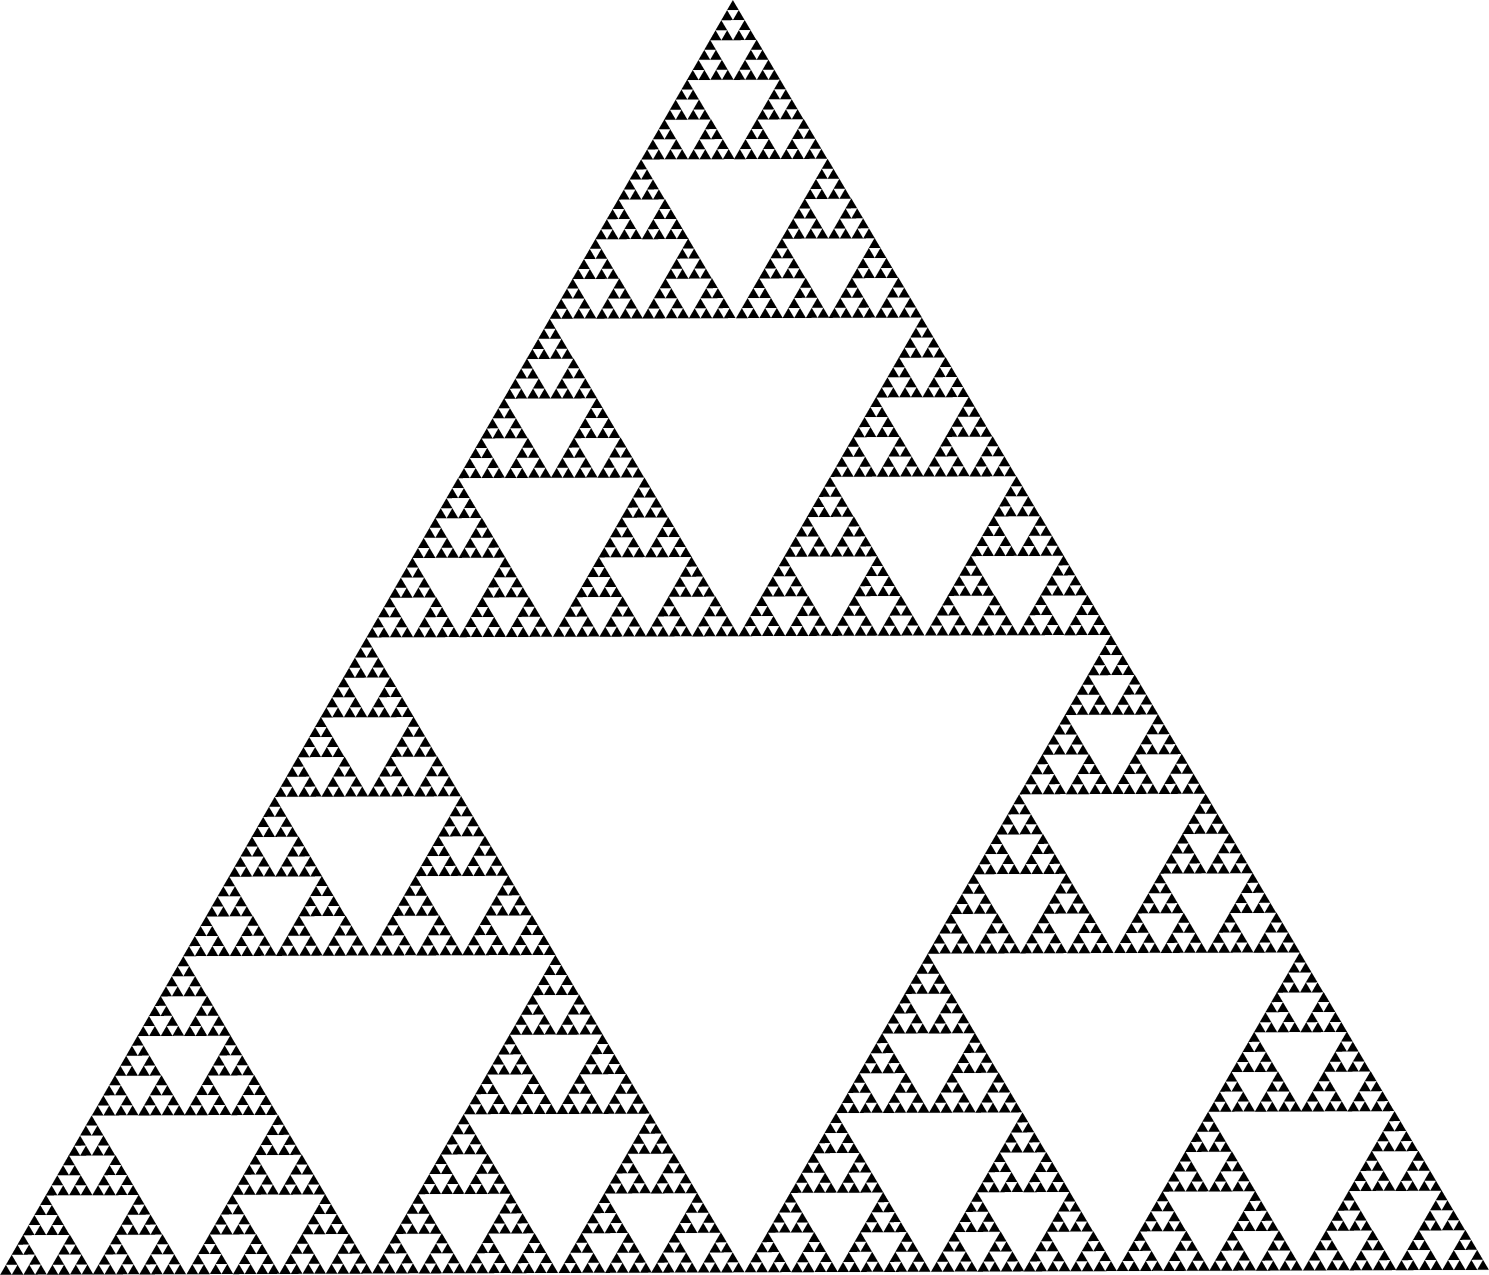
\includegraphics[width=0.8\textwidth]{figures/sierpinski_triangle}
  \caption{Sierpinski-Dreieck: Ein klassisches Fraktal.}
  \label{fig:sierpinski}
\end{figure}

Zwei Abbildungen nebeneinander werden mit \texttt{subcaption}
und der \texttt{subfigure}-Umgebung gesetzt, wie
Abbildung~\ref{fig:fraktale} zeigt. Auf die Teilabbildungen kann
gezielt verwiesen werden: Abbildung~\ref{fig:hilbert} zeigt die
Hilbert-Kurve, Abbildung~\ref{fig:gosper} die Gosper-Kurve.

\begin{figure}[htbp]
  \centering
  \begin{subfigure}[b]{0.48\textwidth}
    \centering
    
\includegraphics[width=\textwidth]{figures/hilbert_kurve}
    \caption{Hilbert-Kurve\footnotemark}
    \label{fig:hilbert}
  \end{subfigure}
  \hfill
  \begin{subfigure}[b]{0.48\textwidth}
    \centering
    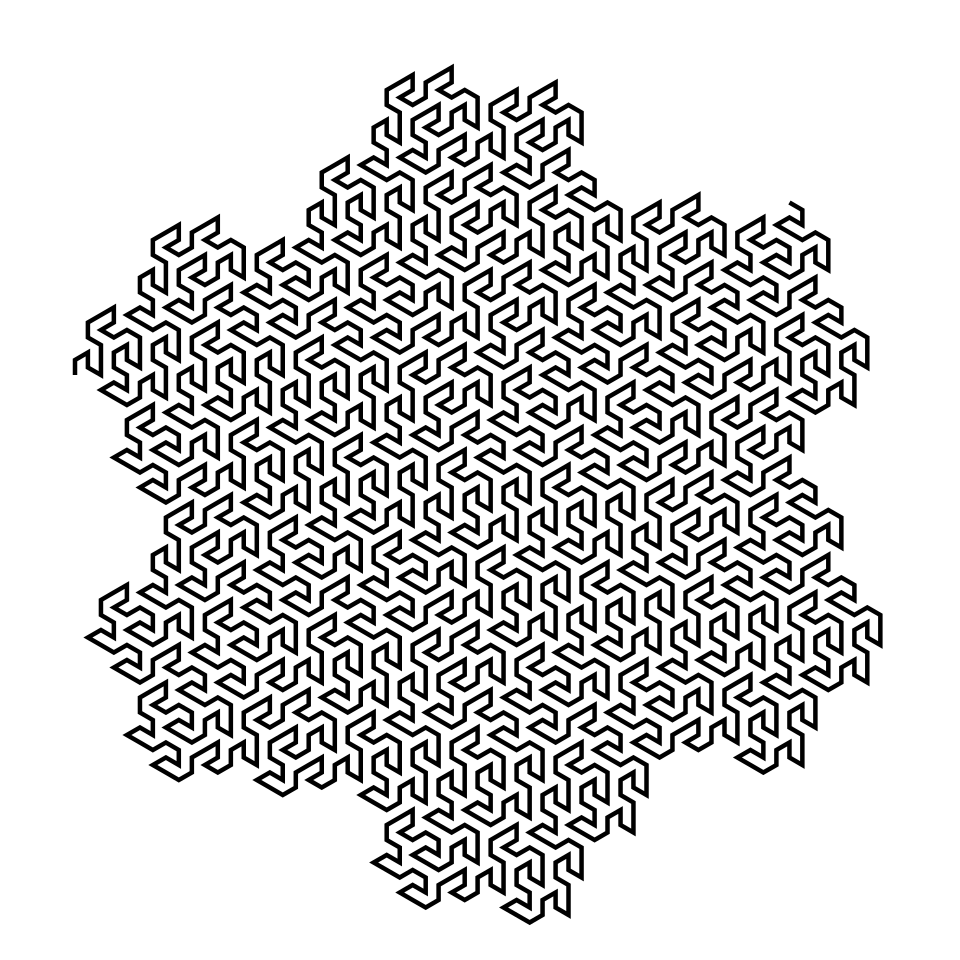
\includegraphics[width=\textwidth]{figures/gosper_kurve}
    \caption{Gosper-Kurve}
    \label{fig:gosper}
  \end{subfigure}
  \caption{Zwei fraktale Kurven.}
  \label{fig:fraktale}
\end{figure}
\footnotetext{Grafik: Alfred Nussbaumer,
  Lizenz: \href{https://creativecommons.org/licenses/by-sa/3.0/}{CC BY-SA 3.0}.}


\section{Tabellen}
\label{sec:tabellen}

Tabellen werden mit dem \texttt{booktabs}-Paket gesetzt.
Tabelle~\ref{tab:vergleich} vergleicht exemplarisch drei
kryptographische Verfahren.

\begin{table}[htbp]
  \centering
  \caption{Vergleich kryptographischer Verfahren}
  \label{tab:vergleich}
  \begin{tabular}{@{} llll @{}}
    \toprule
    Verfahren  & Typ         & Schlüssellänge & Standardisiert \\
    \midrule
    AES-256    & symmetrisch & 256\,Bit       & NIST FIPS 197  \\
    RSA-2048   & asymmetrisch & 2048\,Bit     & PKCS\#1        \\
    Ed25519    & asymmetrisch & 256\,Bit      & RFC 8032       \\
    \bottomrule
  \end{tabular}
\end{table}

Wichtige Regeln für Tabellen: keine vertikalen Linien,
keine doppelten horizontalen Linien, und \emph{nie} \verb|\hline|
bei Verwendung von \texttt{booktabs} \cite{Rechenberg2003}.

\section{Code-Listings}
\label{sec:listings}

Listing~\ref{lst:fibonacci} zeigt eine Beispiel-Implementierung der Fibonacci-Funktion in Java.

\begin{lstlisting}[language=Java,
                   caption={Fibonacci-Funktion mit Rekursion},
                   label={lst:fibonacci}]
public class FibonacciRecursion {
    static int fibonacci(int n) {
        if (n <= 1)
            return n;
        return fibonacci(n - 1) + fibonacci(n - 2);
    }

    public static void main(String[] args) {
        int n = 10; // Change this value as needed
        for (int i = 0; i < n; i++) {
            System.out.print(fibonacci(i) + " ");
        }
    }
}
\end{lstlisting}

Längere Quellcodes (mehr als eine Seite) sollten in den Anhang
ausgelagert werden (siehe Anhang~\ref{app:code}).

\section{Querverweise}
\label{sec:querverweise}

Querverweise werden mit \verb|\ref{}| gesetzt. Dem Befehl wird
stets ein erklärender Begriff vorangestellt und ein
nicht-trennbares Leerzeichen (\verb|~|) verwendet:

\begin{itemize}
  \item Kapitel: Kapitel~\ref{ch:grundlagen}
  \item Abschnitt: Abschnitt~\ref{sec:krypto}
  \item Abbildung: Abbildung~\ref{fig:hilbert}
  \item Tabelle: Tabelle~\ref{tab:vergleich}
  \item Listing: Listing~\ref{lst:fibonacci}
  \item Anhang: Anhang~\ref{app:code}
\end{itemize}

Kapitel~\ref{ch:grundlagen} legt die Grundlagen dar.

% ------------------------------------------------------------
\chapter{Fazit und Ausblick}
\label{ch:fazit}
% ------------------------------------------------------------

\section{Zusammenfassung der Ergebnisse}

Das Fazit fasst die Ergebnisse der Arbeit prägnant zusammen und
bewertet sie kritisch. Welche Forschungsfragen konnten beantwortet
werden? Welche bleiben offen?

\section{Ausblick}

Der Ausblick benennt weiterführende Fragestellungen und zeigt
mögliche Anschlussarbeiten auf.

% ============================================================
%  LITERATURVERZEICHNIS
% ============================================================
\backmatter

\printbibliography[heading=bibintoc]
% heading=bibintoc: trägt das Literaturverzeichnis ins Inhaltsverzeichnis ein

% ============================================================
%  ANHANG
% ============================================================
\appendix

\chapter{Vollständiger Quellcode}
\label{app:code}

Umfangreiche Quellcodes, die den Lesefluss im Haupttext stören
würden, werden hier im Anhang abgedruckt.

\begin{lstlisting}[language=Python,
                   caption={Erweitertes Verschlüsselungsbeispiel},
                   label={lst:erweiterung}]
def caesar_decrypt(text: str, shift: int) -> str:
    """Entschlüsselt einen mit Caesar verschlüsselten Text."""
    return caesar_encrypt(text, -shift)

if __name__ == "__main__":
    geheimtext = caesar_encrypt("Hallo Welt", 3)
    print(f"Verschlüsselt: {geheimtext}")
    print(f"Entschlüsselt: {caesar_decrypt(geheimtext, 3)}")
\end{lstlisting}

\chapter{Weitere Anhänge}
\label{app:b}

Weitere Materialien wie Fragebögen, Messreihen oder Evaluations-
daten können hier eingefügt werden.


\end{document}
